\graphicspath{{images/}}

\section{\thesection~Methods}
\label{sec:methods}

\subsection{\thesubsection~Subsection}

\begin{Figure}
  \centering
  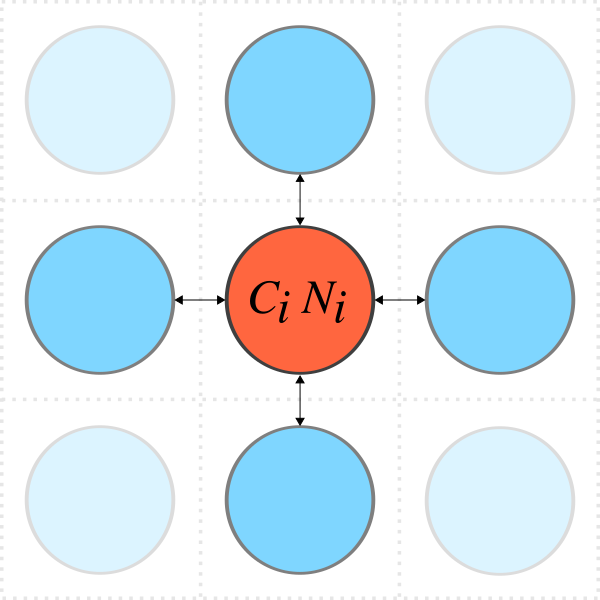
\includegraphics[width=\linewidth]{comp_model/comp_model_schematic}
  \captionof{figure}{\textbf{Schematic of the modelling approach.}
    Each circle represents a culture, indexed \(i\), growing in a grid
    on solid agar. Arrows represent the diffusion of nutrients in the
    network of cultures. \(C_{i}\) - amount of cells; \(N_{i}\) -
    amount of nutrients; darker blue circles - neighbourhood of
    culture i: \(\delta_{i}\).}
  \label{fig:comp_model_schematic}
\end{Figure}


\begin{Figure}
  \centering
  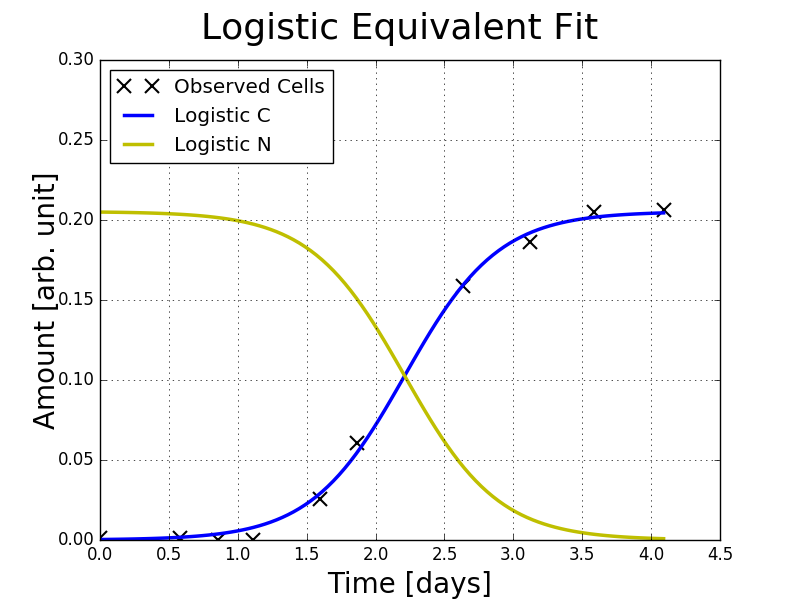
\includegraphics[width=\linewidth]{correction/log_eq_fit}
  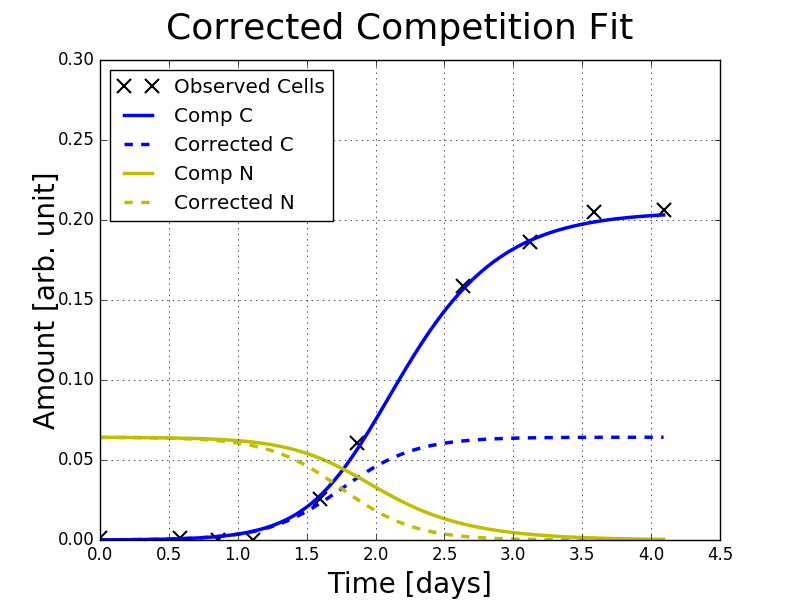
\includegraphics[width=\linewidth]{correction/comp_correction}
  \captionof{figure}{\textbf{Using the competition model to correct
      for competition.} Fits are to culture (R10, C3) of P15 which
    grew faster and reached a higher final cell density than its
    neighbours (not shown). According to the competition model, this
    is because it competed for more nutrients than its neighbours. To
    reach the same final cell density, the logistic equivalent model
    requires a higher amount of starting nutrients and a different
    amount for each culture. The correction to the competition model
    simulates how growth would have appeared without competition and
    allows us to return parameters \(r\) and \(K\) of the logistic
    model.}
  \label{fig:correction}
\end{Figure}

%%% Local Variables:
%%% mode: latex
%%% TeX-master: "report"
%%% End:
